\documentclass[letterpaper, 11pt]{article}
\usepackage{latexsym}
\usepackage{amssymb}
\usepackage{times}
%\usepackage[in]{fullpage}
\usepackage{amsmath,amsfonts,amsthm}
\usepackage{graphicx}
\usepackage{mathtools}
\DeclarePairedDelimiter{\ceil}{\lceil}{\rceil}
\usepackage{listings}
\usepackage{hyperref}

%\documentclass[11pt]{article}
%\pagestyle{myheadings}
%\usepackage[ruled,nothing]{algorithm}
%\usepackage{algorithmic}
%\usepackage[dvips]{epsfig,graphicx}
%\numberwithin{equation}{section}

\bibliographystyle{plain}

\newenvironment{newalgo}[2]{\begin{algorithm}

\caption{\textsc{#1}}\label{#2}

\begin{algorithmic}[1]}{\end{algorithmic}\end{algorithm}}



\newcommand{\gm}{\gamma}
\newcommand{\wh}{\widehat}
\newcommand{\rep}{representation}
\newcommand{\rv}{random variable}
\newcommand{\la}{\lambda}
\newcommand{\wt}{\widetilde}
\newcommand{\st}{such that}
\newcommand{\slvary}{slowly varying}
\newcommand{\ma}{moving average}
\newcommand{\regvary}{regularly varying}
\newcommand{\asy}{asymptotic}
\newcommand{\ts}{time series}
\newcommand{\id}{infinitely divisible}
\newcommand{\seq}{sequence}
\newcommand{\fidi}{finite dimensional \ds}

\newcommand{\ble}{\begin{lemma}}
\newcommand{\ele}{\end{lemma}}
\newcommand{\bfX}{{\bf X}}
\newcommand{\pro}{probabilit}
\newcommand{\BX}{{\bf X}}
\newcommand{\BY}{{\bf Y}}
\newcommand{\BZ}{{\bf Z}}
\newcommand{\BV}{{\bf V}}
\newcommand{\BW}{{\bf W}}
\newcommand{\reals}{{\mathbb R}}
\newcommand{\bbr}{\reals}

\newcommand{\balpha}{\mbox{\boldmath$\alpha$}}
\newcommand{\bbeta}{\mbox{\boldmath$\beta$}}
\newcommand{\bmu}{\mbox{\boldmath$\mu$}}
\newcommand{\tbmu}{\mbox{\boldmath${\tilde \mu}$}}
\newcommand{\bEta}{\mbox{\boldmath$\eta$}}


\def \br#1{\left \{#1 \right \}}
\def \pr#1{\left (#1 \right)}

\newcommand{\Gm}{\Gamma}
\newcommand{\ep}{\epsilon}


\newtheorem{lemma}{Lemma}[section]
\newtheorem{figur}[lemma]{Figure}
\newtheorem{theorem}[lemma]{Theorem}
\newtheorem{proposition}[lemma]{Proposition}
\newtheorem{definition}[lemma]{Definition}
\newtheorem{corollary}[lemma]{Corollary}
\newtheorem{example}[lemma]{Example}
\newtheorem{exercise}[lemma]{Exercise}
\newtheorem{remark}[lemma]{Remark}
\newtheorem{fig}[lemma]{Figure}
\newtheorem{tab}[lemma]{Table}
\newtheorem{fact}[lemma]{Fact}
\newtheorem{test}{Lemma}
\newtheorem{algorithm}[lemma]{Algorithm}

\newcommand{\play}{\displaystyle}

\newcommand{\ms}{measure}
\newcommand{\beao}{\begin{eqnarray*}}
\newcommand{\eeao}{\end{eqnarray*}\noindent}
\newcommand{\beam}{\begin{eqnarray}}
\newcommand{\eeam}{\end{eqnarray}\noindent}

\newcommand{\halmos}{\hfill\mbox{\qed}\\}
\newcommand{\fct}{function}
\newcommand{\ins}{insurance}
\newcommand{\ds}{distribution}

\newcommand{\one}{{\bf 1}}
\newcommand{\eid}{\buildrel{\rm d}\over {=}}
\newcommand {\Or}{\rm ORDER}
\newcommand {\In}{\rm INTER}

\newcommand{\bbd}{{\mathbb D}}
\newcommand{\vi}{$V_{ij}$ }
\newcommand{\rr}{R^{\prime\prime}}
%\newcommand{\R}{R^\prime}
\newcommand{\ci}{\frac{1}{c}}
\newcommand{\Vi}{V(n)}
\newcommand{\dR}{\mathcal R}
\newcommand{\md}[1]{\left(\ \rm{mod}\ \it{#1}\right)}
\newcommand{\So}{s}
%\begin{document}
%\def\DoubleSpace{\baselineskip=24pt}
%\DoubleSpace \sloppy

\begin{document}



\title{ Capital One Challenge Submission\\by\\Nikhil Kulkarni\\MS in Compter Science\\Johns Hopkins University \\ nkulkar7@jhu.edu}

	
\maketitle
Dependencies can be found at the top of the file.
which are sklearn, tabulate, glob, scipy, matplotlib, pandas, numpy.	
\newpage
\section*{ Problem 1 }
\subsection*{Programmatically download and load into your favorite analytical tool the trip data for September 2015}
Done. Please check $get\_file\_content()$ mehtod in $submission.py$ 
\subsection*{Report how many rows and columns of data you have loaded}
Number of rows: $1494926$\\
Number of columns:  $21$

\newpage
\section*{ Problem 2 }
\subsection*{Plot a histogram of the number of the trip distance ("Trip Distance")}
\begin{figure}[h]
	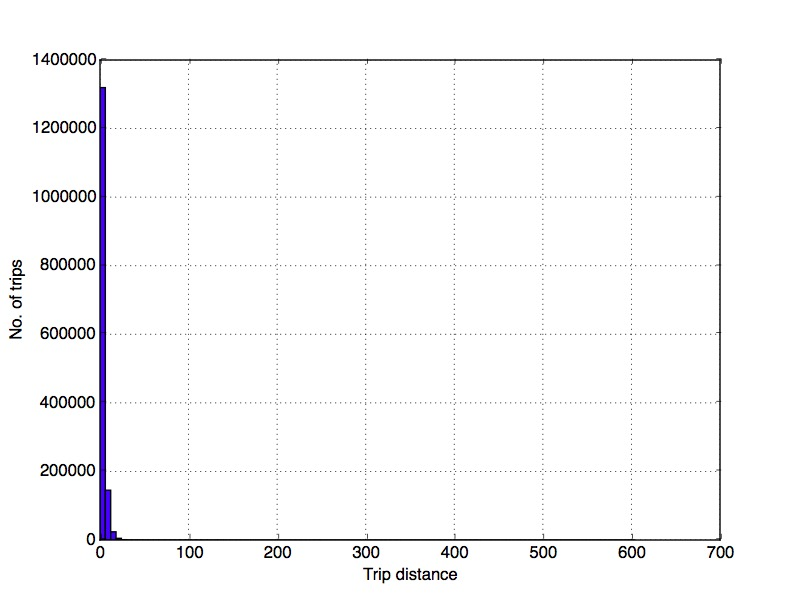
\includegraphics[width=3.5in]{Question2a.jpg}
\end{figure}
\begin{figure}[h]
	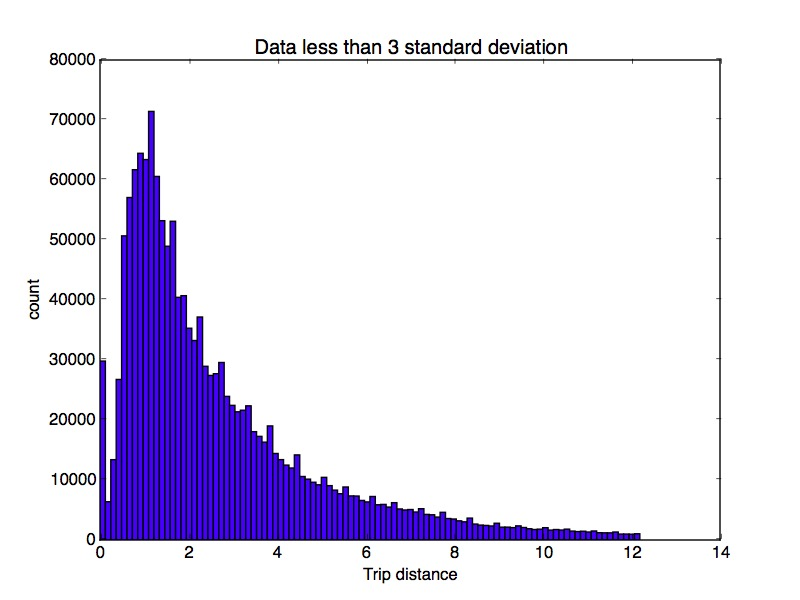
\includegraphics[width=3.5in]{Question2b.jpg}
\end{figure}
\subsection*{Report any structure you find and any hypotheses you have about that structure}
There are a lot of trip with distance on the lower side and lot less rides with distance greater than 80 miles.
The structure can be a normal distribution If we remove the exteme points. We can see that the distribution is normal if we remove points above 3 std deviations.
The number of rides decrease as we go futher and we have a long tail.\\

\subsubsection*{Hypothesis}


Since the Green taxis are not allowed inside the manhatten, it unlikely that people are using green taxis for intercity short travels. The only reason people are using taxis for shorter distance could be to get to nearest metro/train station. It might be the case that the nearest train/metro station is outside manhatten and people prefer green taxis to get there. Also, It might also be the case that most people are living within 12 miles from their work place from manhatten but in the outskirts(and hence green taxis instead of yellow). 

\newpage
\section*{ Problem 3 }
\subsection*{Report mean and median trip distance grouped by hour of day}
Hour \quad    Mean distance\quad   Median distance\\
------\quad  ---------------\quad  -----------------\\
0\quad\quad\quad\quad        3.11528\quad\quad\quad\quad               2.2\\
1          \quad\quad\quad\quad3.01735               \quad\quad\quad\quad2.12\\
2          \quad\quad\quad\quad3.04618               \quad\quad\quad\quad2.14\\
3          \quad\quad\quad\quad3.21295               \quad\quad\quad\quad2.2\\
4          \quad\quad\quad\quad3.52656               \quad\quad\quad\quad2.36\\
5          \quad\quad\quad\quad4.13347               \quad\quad\quad\quad2.9\\
6          \quad\quad\quad\quad4.05515               \quad\quad\quad\quad2.84\\
7          \quad\quad\quad\quad3.28439               \quad\quad\quad\quad2.17\\
8          \quad\quad\quad\quad3.04845               \quad\quad\quad\quad1.98\\
9          \quad\quad\quad\quad2.99911               \quad\quad\quad\quad1.96\\
10          \quad\quad\quad\quad2.94448               \quad\quad\quad\quad1.92\\
11          \quad\quad\quad\quad2.91202               \quad\quad\quad\quad1.88\\
12          \quad\quad\quad\quad2.90306               \quad\quad\quad\quad1.89\\
13          \quad\quad\quad\quad2.87829               \quad\quad\quad\quad1.84\\
14          \quad\quad\quad\quad2.8643                \quad\quad\quad\quad1.83\\
15          \quad\quad\quad\quad2.85704               \quad\quad\quad\quad1.81\\
16          \quad\quad\quad\quad2.77985               \quad\quad\quad\quad1.8\\
17          \quad\quad\quad\quad2.67911               \quad\quad\quad\quad1.78\\
18          \quad\quad\quad\quad2.65322               \quad\quad\quad\quad1.8\\
19          \quad\quad\quad\quad2.7156                \quad\quad\quad\quad1.85\\
20          \quad\quad\quad\quad2.77705               \quad\quad\quad\quad1.9\\
21          \quad\quad\quad\quad2.99919               \quad\quad\quad\quad2.03\\
22          \quad\quad\quad\quad3.18539               \quad\quad\quad\quad2.2\\
23          \quad\quad\quad\quad3.19154               \quad\quad\quad\quad2.22\\
\subsection*{We'd like to get a rough sense of identifying trips that originate or terminate at one of the NYC area
	airports. Can you provide a count of how many transactions fit this criteria, the average fair, and any other
interesting characteristics of these trips}

One approach could be to use lattitude langitude data and get information about the boundaries of the airport areas. Then by finding how many trips started or ended within that specific area, we can determine the number of trips and other stats.\\
But,  With reference to this link \\
\url{http://www.nyc.gov/html/tlc/downloads/pdf/data_dictionary_trip_records_yellow.pdf}\\
JFK and newark (probably airport areaas have ids 2 and 3)\\
With this info we can just filter the data to get values that are required.
\subsection*{Results}
\textbullet \quad No. of trips to/from airport:  5552\\
\textbullet \quad Avg. fare airport:  48.98\\
\textbullet \quad Avg. total amount airport: 57.21\\

\subsection*{Interesting characteristics}
One interesting fact is that usually in smaller cities the taxis are used heavily in the late night only to travel to airports since the public transport is closed. But with hourly data for airport rides and normal rides, we can see that this distinction is not true. This might be due to the fact that there are enough number of people taking regular rides even in the late night time. Airport taxi traffic is comparable to the normal traffic in the late night.\\
It is interesting to note that average Fare amount is 12.54 while average Total amount is 15.03. But at the airport area these figures are almost 4 times the normal values.
Also, average distance of all airport trips is higher than average distance of all trips. This might be due to the fact that both airports might be having high number of passengers from manhatten area. The histogram of airport trips shows high number of trips for distances lower than ~20 miles. 
\newpage
\section*{ Problem 4 }
\subsection*{Build a derived variable for tip as a percentage of the total fare}
Done.\\
$data['Per\_TIP'] = 100*data.Tip\_amount/data.Total\_amount$


\subsection*{Build a predictive model for tip as a percentage of the total fare. Use as much of the data as you like (or
all of it). We will validate a sample}
I will be considering only following features for the prediction model.\\

"RateCodeID",
"Pickup\_longitude",
"Pickup\_latitude",
"Dropoff\_longitude",
"Dropoff\_latitude",
"Passenger\_count",
"Trip\_distance",
"Fare\_amount",
"Extra",
"MTA\_tax",
"Tolls\_amount",
"Total\_amount",
"Payment\_type",
"Trip\_type "\\

The data is split with test size of 0.25\\

Then the data is scaled using $StandardScaler$ from $sklearn.preprocessing$ package\\

Finally I am testing following classifiers for the predictions.\\

1. Linear regression with no penalty\\

2. Linear regression with l2 normalization\\

3. SVM linear\\
 
4. SVM poly\\
  
5. SVM RBF\\
  
6. Tree regressor\\

Out of these tree regressor works the best. I have printed the performance metrics for this classifier.

\section*{Visualization}

I have built a D3 visualization with of the from the location data to indicate the pick up and drop of points. please find file $index.html$ which has some sample points which I was able to display on the D3 map. \\
for running this file you will need to run a simple http server using python. 
$python -m SimpleHTTPServer$ in the folder where files are extracted.
And then use browser to visit localhost:8000


\end{document}

%%%%%%%%%%%%%%%%%%%%%%%%%%%%%
